\documentclass{scrartcl}
\usepackage[mathletters]{ucs}
\usepackage[utf8x]{inputenc}
\usepackage{amssymb}
\usepackage{amsmath}
\usepackage[usenames]{color}
\usepackage{hyperref}
\usepackage{wasysym}
\usepackage{graphicx}
\usepackage[normalem]{ulem}
\usepackage{enumerate}

\usepackage{listings}

\lstset{ %
basicstyle=\footnotesize,       % the size of the fonts that are used for the code
showspaces=false,               % show spaces adding particular underscores
showstringspaces=false,         % underline spaces within strings
showtabs=false,                 % show tabs within strings adding particular underscores
frame=single,                   % adds a frame around the code
tabsize=2,                      % sets default tabsize to 2 spaces
breaklines=true,                % sets automatic line breaking
breakatwhitespace=false,        % sets if automatic breaks should only happen at whitespace
}


\title{First Camera Mount}
\date{dinsdag 08 december 2020}
\author{}

\begin{document}

\maketitle

		\section{First Camera Mount}

Created Wednesday 28 October 2020



The printing process can be seen in the next picture:

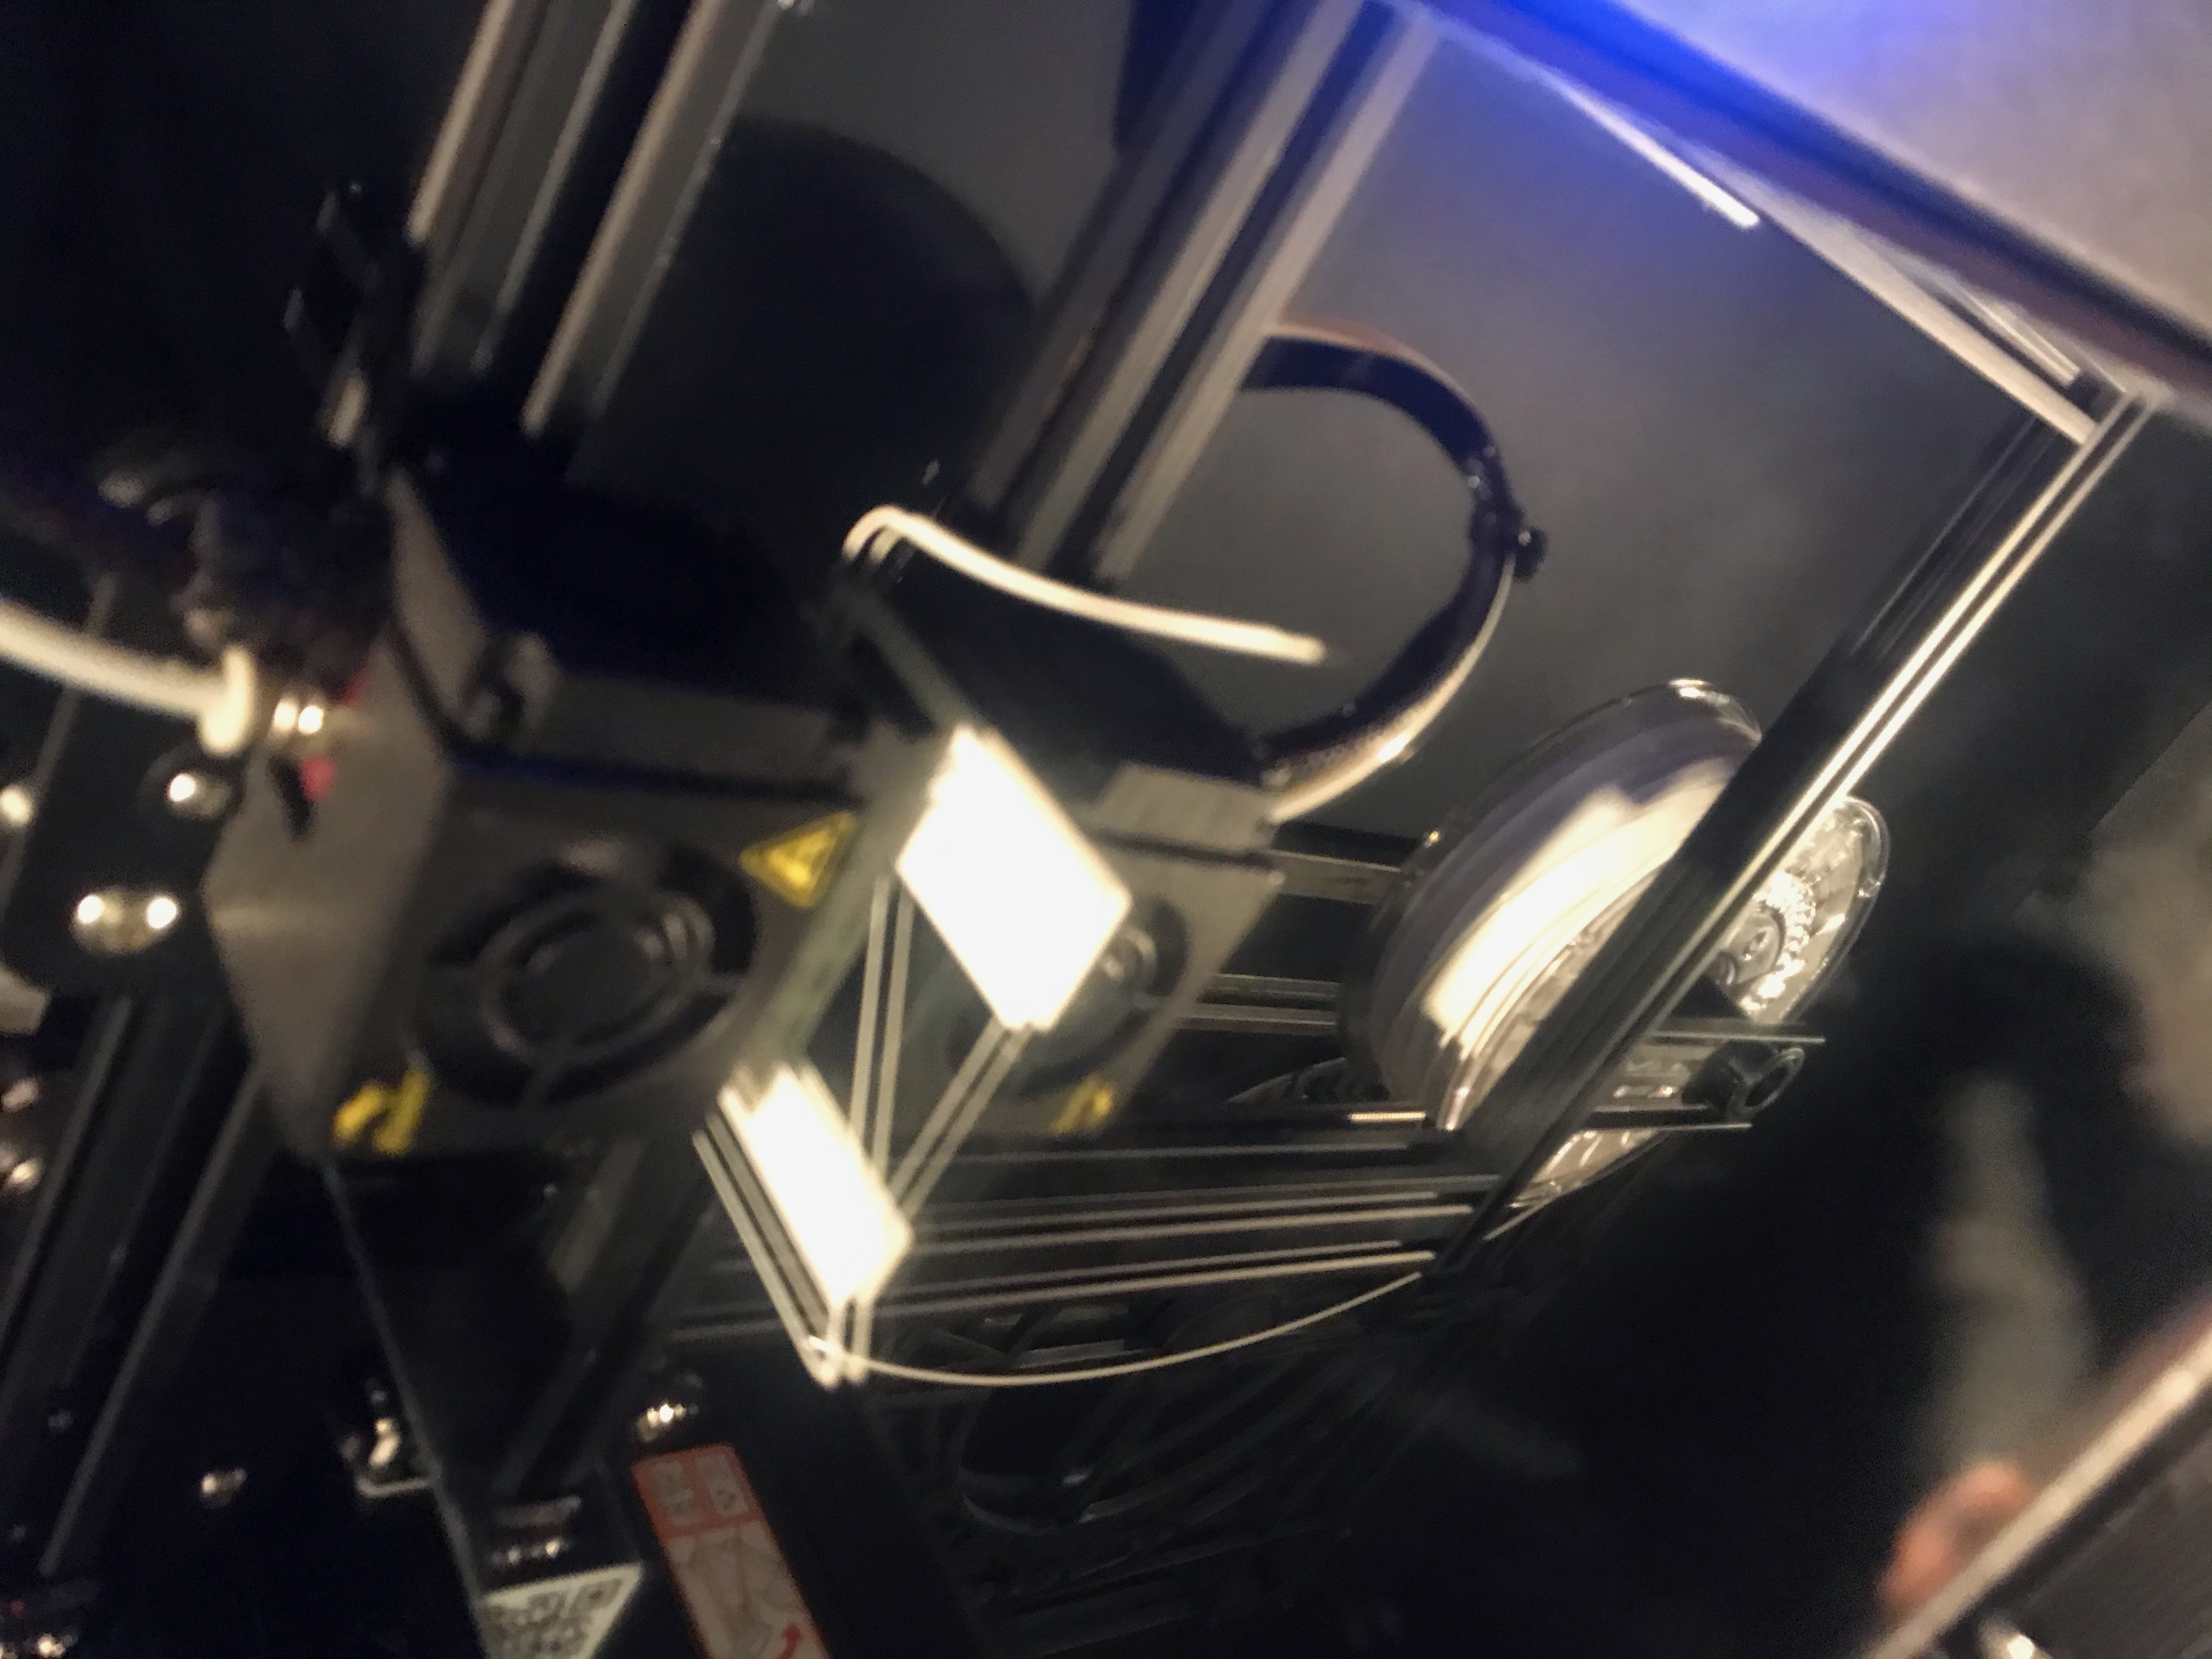
\includegraphics[height=3.125000in, keepaspectratio=true]{./First_Camera_Mount/3D_print_houder.jpeg}



Here PLA is used to print on a temperature of 200 degrees Celcius, on a heated bed of 60 degree Celcius. This is a holder which should support the camera while keeping the tool on the tool holder in place. The result wasn't good due to the print not sticking enough to the printing bed, no other test print was made. There will be another mount designed further in the process when the \href{../Light.tex}{Light}  is more sorted out and the \href{../Tool_Holder.tex}{Tool Holder} is further developed. Now only the \href{../Tool_Holder/Simple_holder.tex}{Simple holder} was in use with the first \href{../Light/Desk_Lamp_Test.tex}{Desk Lamp Test.} 



The full setup can be seen in the following picture: Here the 3D printed plate goes under the postits to get consistent placement of the tool to the camera. 

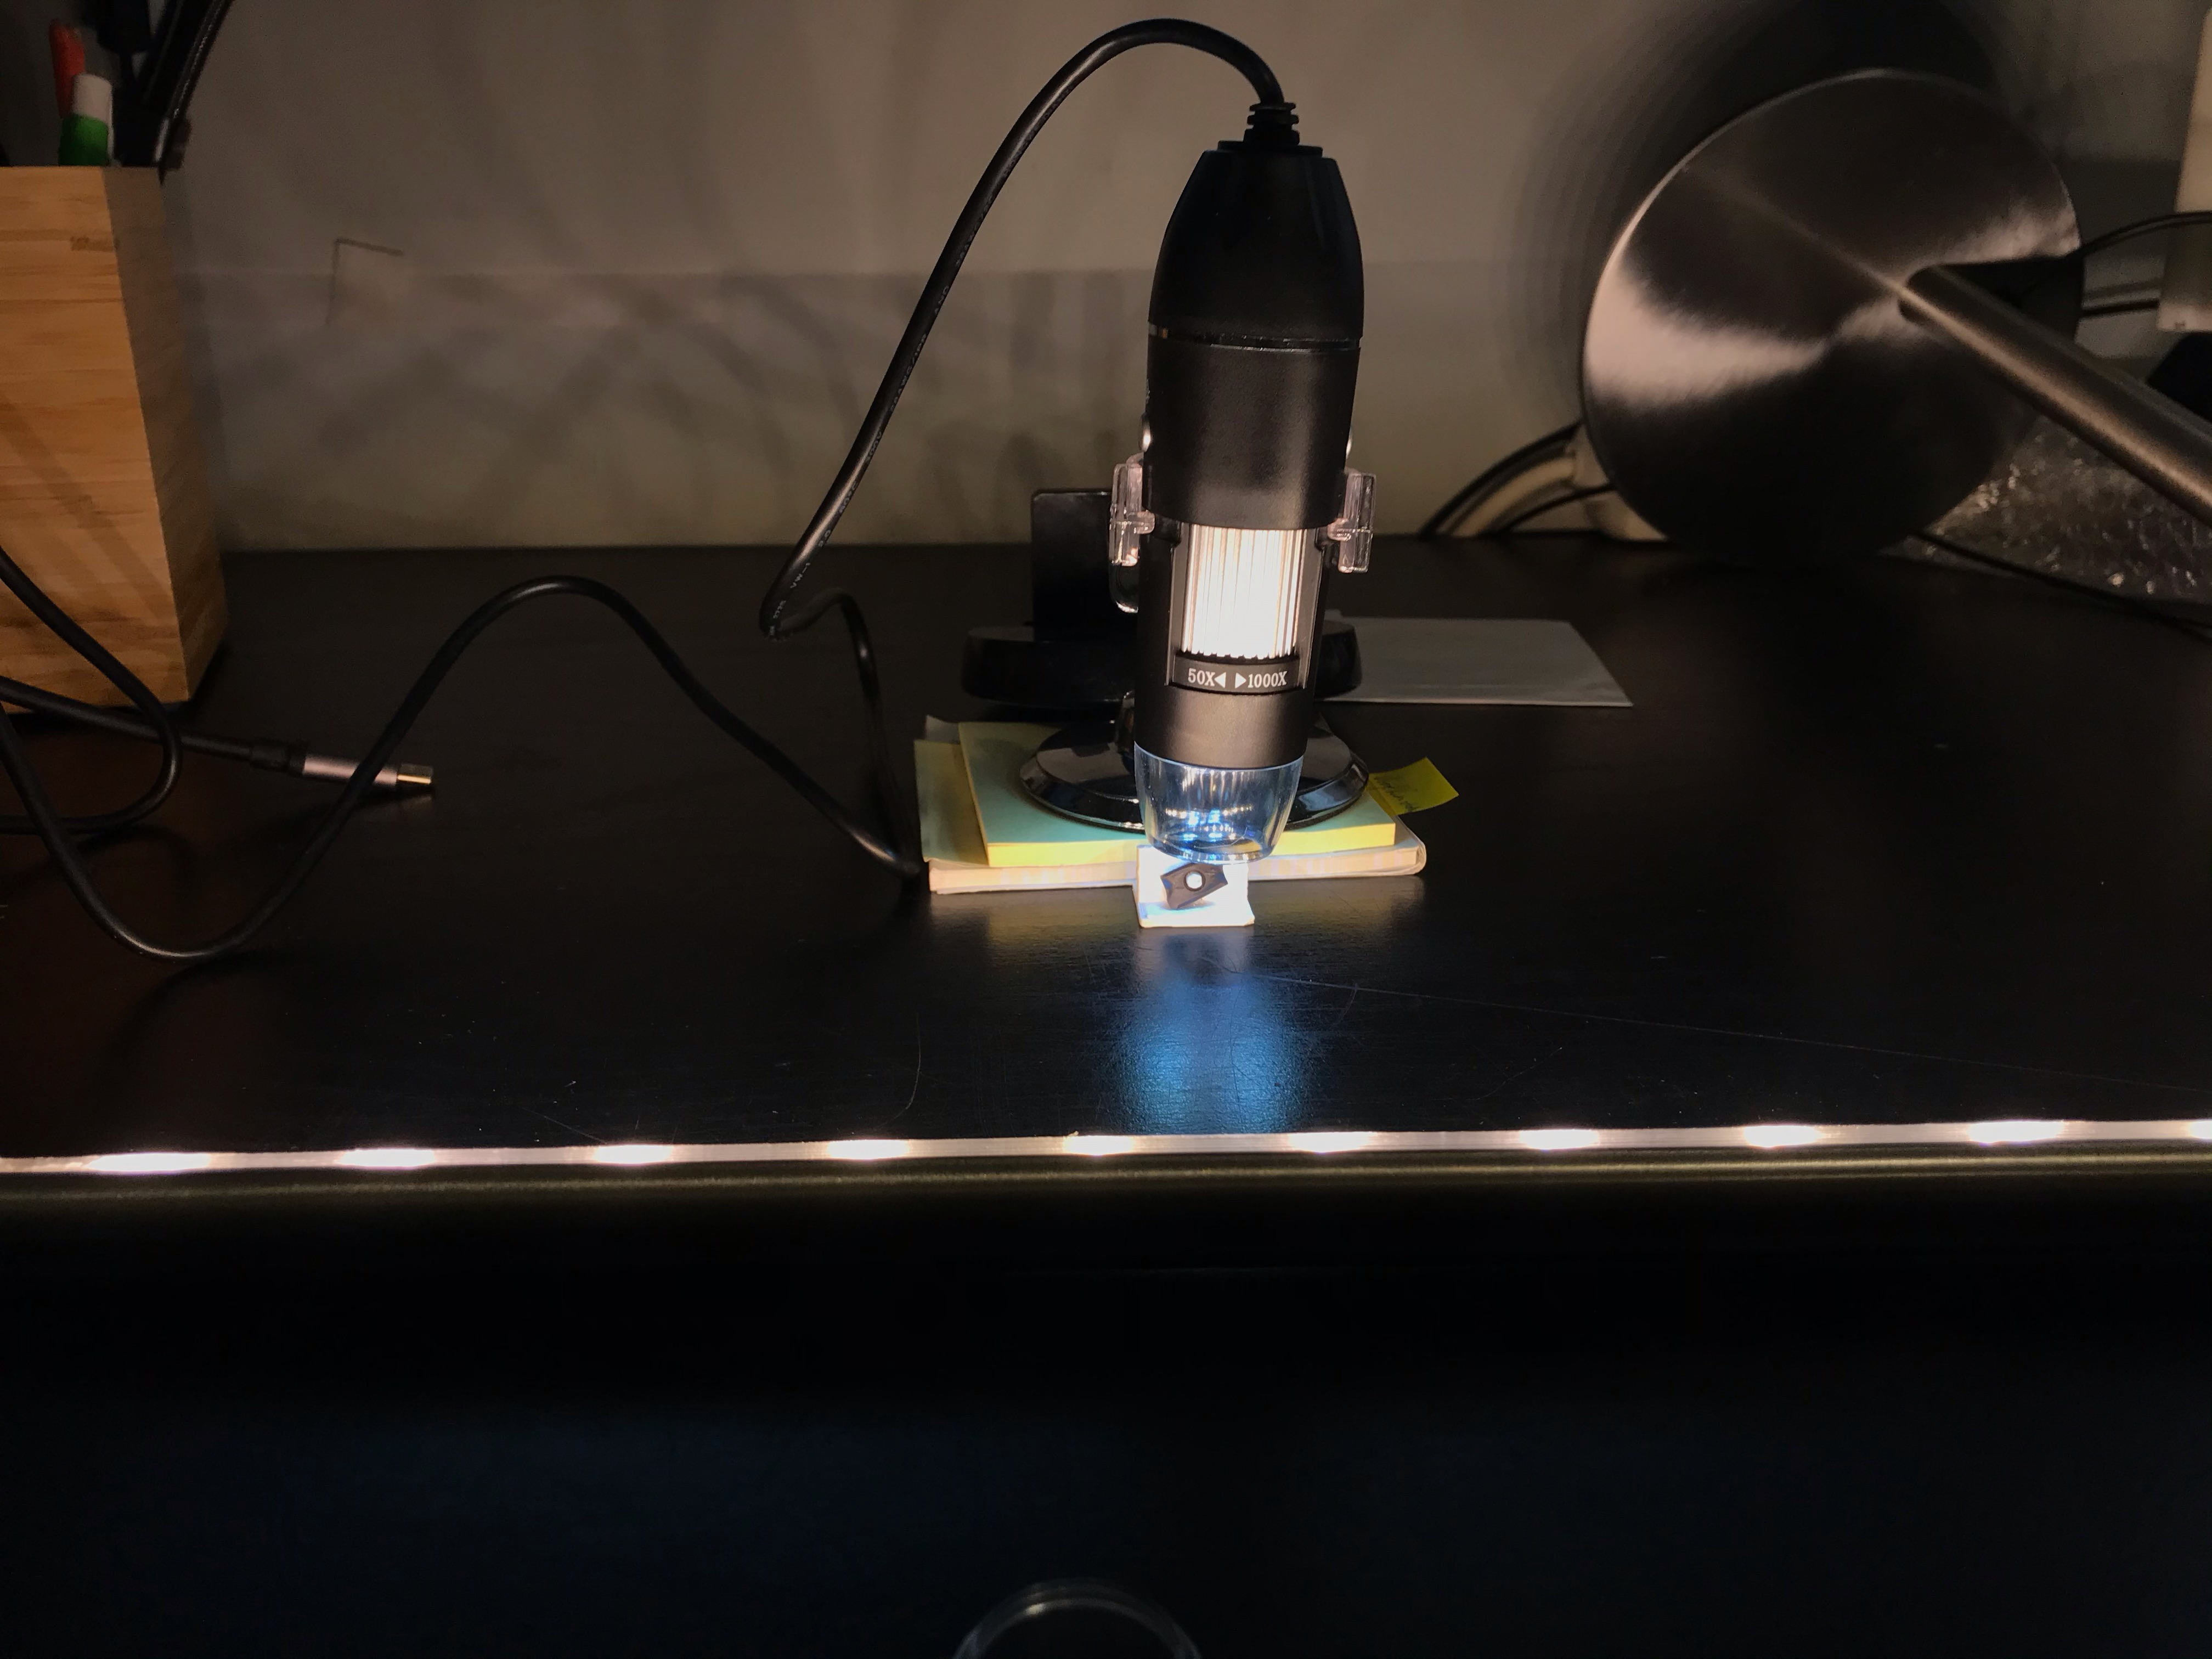
\includegraphics[height=3.125000in, keepaspectratio=true]{./First_Camera_Mount/eerste_setup_andere_richting.jpeg}





\end{document}
